\chapter{Prospettiva sulla programmazione parallela}
\section{4 passi nella creazione di un programma parallelo}
\begin{figure}[H]
    \centering 
    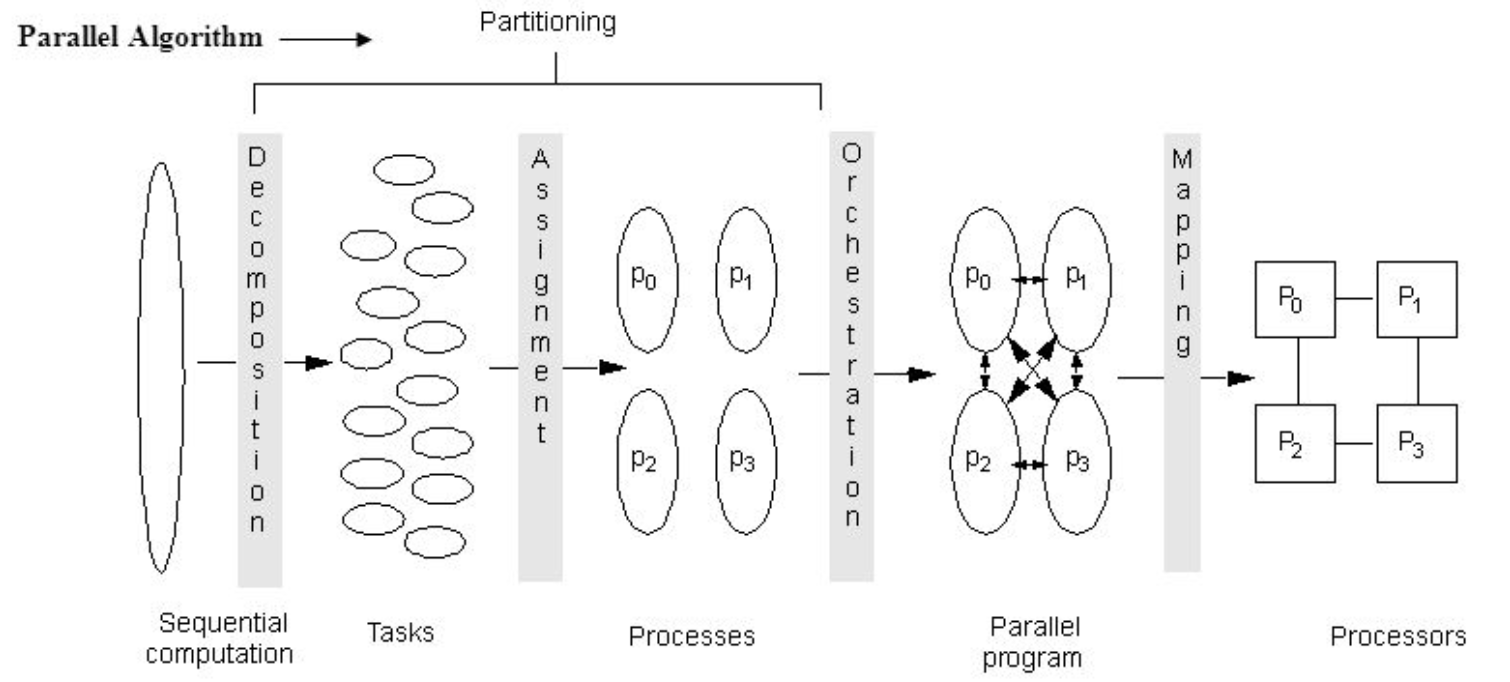
\includegraphics[scale=0.5]{img/4steps.png}
\end{figure}
\begin{enumerate}
    \item \textbf{Decomposizione}: si divide il
    problema in sotto-problemi
    più piccoli.
    \item \textbf{Assegnazione}: si assegna ogni
    sotto-problema ad un 
    processore.
    \item \textbf{Orchestrazione}: si sincronizzano i processori.
    \item \textbf{Mapping}: si ricombinano i risultati.
\end{enumerate}

\section{Capire il problema e il programma}
Indubbiamente, il primo passo nello sviluppo di software
parallelo è comprendere a fondo il problema che si desidera
risolvere in parallelo. Se si parte da un programma
seriale esistente, questo necessita anche di una profonda
comprensione del codice attuale. Questo aspetto è cruciale
poiché la natura del problema influisce sulla fattibilità
di un approccio parallelo e su come esso potrebbe essere
strutturato.

Prima di investire tempo nello sviluppo di una soluzione
parallela, è essenziale determinare se il problema
in questione è adatto alla parallelizzazione.
Non tutti i problemi possono beneficiare dell'esecuzione
parallela, e riconoscere questo aspetto in anticipo
può risparmiare tempo e risorse significative.

Un chiaro esempio di problema che può essere
parallelizzato è il calcolo dell'energia potenziale per
ciascuna di diverse migliaia di conformazioni indipendenti
di una molecola. Una volta completati tutti i calcoli,
rimane il compito di trovare la conformazione con l'energia
minima.

Un esempio tipico di problema non parallelizzabile è
il calcolo della serie di Fibonacci
utilizzando la formula:
\[ F(k + 2) = F(k + 1) + F(k) \]

Questo rappresenta un problema non parallelizzabile
perché il calcolo della sequenza di Fibonacci, come
mostrato, implica calcoli dipendenti piuttosto che
indipendenti.

\begin{itemize}
    \item Il calcolo del valore \( F(k + 2) \)
    utilizza i valori di \( F(k + 1) \) e \( F(k) \).
    Questi tre termini non possono essere calcolati
    indipendentemente e, quindi, non possono essere
    eseguiti in parallelo.
\end{itemize}

La dipendenza diretta tra i termini consecutivi della
serie impedisce qualsiasi decomposizione che permetta
un'elaborazione parallela efficace, dimostrando così
le limitazioni di alcuni tipi di problemi rispetto alla
parallelizzazione.


\begin{itemize}
    \item Questo problema si presta bene al processo parallelo perché ogni conformazione molecolare può essere determinata indipendentemente dalle altre.
    \item Il compito successivo di identificazione della conformazione di energia minima è anch'esso parallelizzabile, in quanto coinvolge il confronto di risultati che possono essere elaborati in parallelo.
\end{itemize}

Questo esempio illustra come i compiti possono essere decomposti ed eseguiti in parallelo, accelerando significativamente il processo di calcolo complessivo nelle applicazioni adatte.

\subsection{Identificazione dei Punti Critici in un Programma}

\textbf{Identificare i Hotspots del Programma:}
Identificare i \textit{hotspots}, ovvero le zone dove il programma
compie la maggior parte del lavoro, è essenziale. Molti
programmi scientifici e tecnici concentrano gran
parte delle loro operazioni in poche aree critiche.
L'uso di strumenti di profilazione e analisi delle
prestazioni è quindi cruciale per individuare queste aree.
Concentrarsi sulla parallelizzazione di questi hotspots
può aumentare notevolmente l'efficienza del programma,
mentre le sezioni che utilizzano meno \texttt{CPU}
possono essere
trascurate in questa fase iniziale.

\textbf{Identificare i Colli di Bottiglia nel Programma:}
È importante riconoscere le aree del programma che
sono sproporzionatamente lente o che causano interruzioni
o ritardi nel lavoro che potrebbe essere parallelizzato.
Spesso, operazioni come l'\texttt{I/O} sono responsabili di questi
rallentamenti. Modificare la struttura del programma
o adottare un diverso algoritmo può aiutare a ridurre
o eliminare queste inefficienze,
migliorando così le prestazioni complessive.

\textbf{Identificare gli Inibitori al Parallelismo:}
Un altro aspetto fondamentale è identificare gli inibitori
al parallelismo. La dipendenza dai dati è un esempio
comune di questi ostacoli, come dimostrato dalla sequenza
di Fibonacci. Queste dipendenze creano una situazione in
cui i calcoli devono essere eseguiti in un ordine
specifico, il che limita le opportunità di eseguire
il processo in parallelo.

\textbf{Esplorare Altri Algoritmi:} Infine,
l'esplorazione di altri algoritmi può rappresentare
la considerazione più importante nella progettazione
di un'applicazione parallela. Trovare un algoritmo più
adatto al parallelismo può spesso offrire soluzioni più
efficienti e performanti.

\section{Decomposizione}
Identificare la concorrenza in un programma
e decidere il livello al quale sfruttarla è
fondamentale per ottimizzare l'esecuzione parallela.
Questo processo inizia con la suddivisione del calcolo
in compiti che possono essere distribuiti tra diversi processi. È importante notare che i compiti possono diventare disponibili dinamicamente e che il numero di compiti disponibili può variare nel tempo.

L'obiettivo principale è avere abbastanza compiti per
mantenere i processi occupati, ma non troppi; infatti,
il numero di compiti disponibili in un dato momento
rappresenta il limite superiore della velocità di
esecuzione che può essere raggiunta. Troppi
compiti potrebbero sovraccaricare i processi
e diminuire l'efficienza complessiva, mentre
troppo pochi compiti potrebbero lasciare alcune
risorse inutilizzate, riducendo la performance.

Per quanto riguarda la suddivisione del lavoro
computazionale tra i task paralleli, esistono
due metodi fondamentali: la decomposizione per
dominio e la decomposizione funzionale. La
\textbf{decomposizione per dominio} implica
dividere i dati su cui opera il programma in parti
che possono essere processate in parallelo, mentre
la \textbf{decomposizione funzionale} comporta
la divisione delle funzioni del programma in sotto-funzioni
che possono essere eseguite contemporaneamente.

\subsection{Decomposizione per Dominio}
La decomposizione per dominio è una tecnica
comune per suddividere il lavoro in un programma
parallelo. Questo approccio prevede la divisione
dei dati in parti che possono essere processate
indipendentemente. Questo metodo è particolarmente
utile quando i dati sono indipendenti tra loro
e possono essere elaborati senza interazioni
tra i processi.

Un esempio di decomposizione per dominio è
l'analisi di un'immagine in cui ogni pixel
può essere elaborato indipendentemente dagli
altri. In questo caso, l'immagine può essere
divisa in sezioni che possono essere processate
in parallelo, accelerando notevolmente il
processo di analisi.

La decomposizione per dominio può essere
svolta in diversi modi, nel caso mono-dimensionale
si può dividere il lavoro in blocchi di dati
o eseguire il lavoro in modo ciclico.
Nel caso bidimensionale, si può dividere il
lavoro in righe o colonne, o in blocchi di
dimensioni maggiori. Anche nel caso bidimensionale
è possibile eseguire il lavoro in modo ciclico.

\subsection{Decomposizione Funzionale}
La decomposizione funzionale è un'altra tecnica
importante per la progettazione di programmi
paralleli. Questo approccio prevede la divisione
delle funzioni del programma in sotto-funzioni
che possono essere eseguite contemporaneamente.
Questo metodo è particolarmente utile quando
le funzioni del programma possono essere
eseguite indipendentemente l'una dall'altra.

Un esempio di decomposizione funzionale è
l'elaborazione di un documento di testo in cui
ogni paragrafo può essere analizzato
indipendentemente dagli altri. In questo caso,
il documento può essere suddiviso in paragrafi
che possono essere processati in parallelo,
accelerando notevolmente il processo di analisi.

\section{Assegnazione}
Nel contesto della programmazione parallela, è cruciale
considerare i compiti come ``cose da fare'' e i thread
come ``lavoratori''. Questa analogia aiuta a visualizzare
la distribuzione del lavoro tra i processi. Ad esempio,
potremmo decidere quale processo calcola le forze su quali
stelle, o quali raggi vengono calcolati da quale processo.
L'obiettivo principale è bilanciare il carico di lavoro,
riducendo i costi di comunicazione e gestione, noto anche
come \textit{load balancing}.

\subsection{Approcci Strutturati alla Divisione dei
Compiti}
Gli approcci strutturati tendono a funzionare bene in
questo contesto:
\begin{itemize}
    \item L'ispezione del codice (\textit{come i loop
    paralleli}) o la comprensione dell'applicazione
    possono guidare la divisione efficace dei compiti.
    \item L'uso di euristiche ben note può facilitare
    questo processo.
    \item Si considerano assegnazioni statiche versus
    dinamiche dei compiti, a seconda della natura e
    delle esigenze dell'applicazione.
\end{itemize}

Come programmatori, tendiamo a preoccuparci prima della partizione, che di solito è indipendente dall'architettura o dal modello di programmazione. Tuttavia, il costo e la complessità nell'uso delle primitive possono influenzare le decisioni.

\subsection{Bilanciamento del Carico}

Il bilanciamento del carico si riferisce alla pratica
di distribuire i compiti tra i processi in modo che tutti
i processi siano costantemente occupati, minimizzando
il tempo di inattività dei processi. Questo aspetto è
fondamentale per le prestazioni dei programmi paralleli.
Ad esempio, se tutti i processi sono soggetti a un punto
di sincronizzazione a barriera, il compito più lento
determinerà le prestazioni complessive.

\subsubsection{Come Raggiungere il Bilanciamento del Carico}
\begin{itemize}
    \item L'assegnazione dinamica del lavoro può
    essere utilizzata per gestire i compiti in modo
    flessibile.
    \item Alcune classi di problemi risultano in squilibri
    di carico anche se i dati sono distribuiti
    uniformemente tra i processi:
    \begin{itemize}
        \item Array sparsi - alcuni processi avranno dati
        effettivi su cui lavorare mentre altri hanno
        prevalentemente ``zeri".
        \item Metodi di griglia adattivi - alcuni processi
        potrebbero dover raffinare la loro mesh mentre
        altri no.
        \item Simulazioni N-body - dove alcune particelle
        possono migrare verso o lontano da un processo.
    \end{itemize}
    \item Quando il lavoro che ogni processo eseguirà
    è intenzionalmente variabile o non prevedibile, può
    essere utile utilizzare un approccio di scheduler -
    task pool. Man mano che ogni processo completa il suo
    lavoro, si mette in coda per ottenere un nuovo pezzo
    di lavoro.
    \item Potrebbe diventare necessario progettare un
    algoritmo che rilevi e gestisca gli squilibri di
    carico man mano che si verificano dinamicamente
    all'interno del codice.
\end{itemize}

\subsection{Granularità nel Calcolo Parallelo}

\subsubsection{Rapporto Computazione/Comunicazione}
Nel calcolo parallelo, la granularità è una misura
qualitativa del rapporto tra computazione e comunicazione.
I periodi di computazione sono tipicamente separati dai
periodi di comunicazione attraverso eventi di
sincronizzazione. Questa distinzione è fondamentale
per comprendere e ottimizzare le prestazioni dei sistemi
paralleli.

\subsubsection{Granularità del Parallelismo}
Il parallelismo può essere classificato in base alla
granularità delle operazioni che vengono eseguite:
\begin{description}
    \item[Fine grain parallelism]
    dove piccole quantità di lavoro computazionale
    sono seguite da eventi di comunicazione, con un
    basso rapporto tra computazione e comunicazione.
    Questo tipo di parallelismo può aiutare a ridurre
    gli overhead dovuti agli squilibri di carico, ma
    potrebbe incrementare gli overhead di comunicazione
    e sincronizzazione.
    \item[Coarse grain parallelism] caratterizzato da
    quantità relativamente grandi di lavoro computazionale
    che intervallano gli eventi di
    comunicazione/sincronizzazione. Questo comporta
    un alto rapporto computazione/comunicazione,
    suggerendo maggiori opportunità di incremento delle
    prestazioni, anche se può essere più difficile
    da bilanciare efficacemente il carico di lavoro.
\end{description}

\subsubsection{Parallelismo Fine o Grossolano?}
La granularità più efficiente dipende dall'algoritmo
specifico e dall'ambiente hardware in cui opera. In molti
casi, l'overhead associato alle comunicazioni e alla
sincronizzazione è elevato rispetto alla velocità di
esecuzione, rendendo vantaggiosa una granularità
grossolana. Tuttavia, il parallelismo fine può essere
utile per ridurre gli overhead dovuti agli squilibri di
carico. La scelta tra granularità fine o grossolana deve
quindi essere ponderata in base alle specifiche esigenze
dell'applicazione e alle caratteristiche del sistema di
calcolo utilizzato.

\section{Orchestrazione}

L'orchestrazione in calcolo parallelo si concentra sulla
strutturazione della comunicazione, sulla sincronizzazione
e sull'organizzazione delle strutture di dati e sulla
programmazione temporale dei compiti. Gli obiettivi
principali di questa fase includono:

\begin{itemize}
    \item Ridurre i costi di comunicazione e
    sincronizzazione.
    \item Preservare la località del riferimento ai dati.
    \item Programmare i compiti in modo da soddisfare
    le dipendenze il più presto possibile.
    \item Ridurre l'overhead della gestione del
    parallelismo.
\end{itemize}

Le scelte in questa fase dipendono dal modello di
programmazione adottato, dall'astrazione della
comunicazione e dall'efficienza delle primitive offerte
dai progettisti di sistemi.

\subsection{Comunicazioni nel Calcolo Parallelo}

\subsubsection{Chi necessita delle comunicazioni?}
La necessità di comunicazioni tra compiti dipende
dalla natura del problema:

\begin{description}
    \item[Non necessita comunicazioni:] Alcuni tipi
    di problemi possono essere decomposti ed eseguiti
    in parallelo senza quasi alcuna necessità di
    condivisione di dati tra i compiti. Ad esempio,
    un'operazione di elaborazione di immagini dove ogni
    pixel in un'immagine in bianco e nero deve avere
    il suo colore invertito. I dati dell'immagine possono
    essere facilmente distribuiti a più compiti che
    agiscono indipendentemente l'uno dall'altro per
    svolgere la loro parte di lavoro. Questi tipi di
    problemi sono spesso chiamati parallelamente
    imbarazzanti perché sono così diretti.
    \item[Necessita comunicazioni:] La maggior parte
    delle applicazioni parallele non è così semplice e
    richiede che i compiti condividano dati tra di loro.
    Ad esempio, un problema di diffusione del calore in
    \texttt{3D} richiede che un compito conosca le
    temperature calcolate dai compiti che hanno dati
    adiacenti. Le modifiche ai dati adiacenti hanno un
    effetto diretto sui dati del compito.
\end{description}

\subsubsection{Fattori importanti nella progettazione
delle comunicazioni inter-task}
\begin{itemize}
    \item \textbf{Costo delle comunicazioni:} La
    comunicazione inter-task implica quasi sempre
    un overhead. I cicli di macchina e le risorse che
    potrebbero essere utilizzati per la computazione
    vengono invece utilizzati per impacchettare e
    trasmettere dati.
    \item \textbf{Latency vs Bandwidth:}
    \begin{itemize}
        \item La \textit{latency} è il tempo necessario
        per inviare un messaggio minimo ($0 byte$) da un
        punto A a un punto B.
        \item La \textit{bandwidth} è la quantità di
        dati che può essere comunicata per unità di tempo,
        comunemente espressa in megabyte/sec o
        gigabyte/sec.
    \end{itemize}
    \item \textbf{Visibilità delle comunicazioni:} Con
    il modello di passaggio di messaggi, le comunicazioni
    sono esplicite e generalmente ben visibili e sotto
    il controllo del programmatore. Con il modello di
    parallelismo sui dati, le comunicazioni spesso
    avvengono trasparentemente per il programmatore,
    particolarmente su architetture a memoria distribuita.
    \item \textbf{Comunicazioni sincrone vs asincrone:}
    Le comunicazioni possono essere sincrone, bloccanti
    o non bloccanti, a seconda delle necessità
    dell'applicazione.
\end{itemize}

\subsubsection{Tipi e Complessità delle Comunicazioni}
Nella progettazione di codici paralleli, è essenziale
determinare quali compiti devono comunicare tra loro.
Queste comunicazioni possono essere implementate sia
in modo sincrono che asincrono e si dividono in due
categorie principali:

\textbf{Comunicazione Punto-a-Punto:} Coinvolge due
compiti specifici dove uno agisce come mittente/produttore
di dati e l'altro come ricevitore/consumatore. Questa
tipologia è ideale per il trasferimento diretto di dati
tra due entità.

\textbf{Comunicazione Collettiva:} Implica la
partecipazione di più di due compiti, generalmente
definiti come membri di un gruppo collettivo. Le varianti
comuni includono:
\begin{itemize}
    \item \textbf{Broadcast:} Dati inviati da un mittente
    a tutti i partecipanti.
    \item \textbf{Scatter:} Dati divisi e inviati a
    diversi ricevitori dallo stesso mittente.
    \item \textbf{Gather:} Dati raccolti da diversi
    mittenti in un singolo ricevitore.
    \item \textbf{Allgather, Reduce, e Allreduce:}
    Operazioni che combinano le funzionalità di raccolta
    e distribuzione dati, con tutti i partecipanti che
    inviano o ricevono dati.
\end{itemize}

\textbf{Sovraccarico e Complessità:} Le comunicazioni
introducono un sovraccarico derivante dalla necessità
di sincronizzare i compiti, impacchettare e trasmettere
dati, e gestire il traffico di rete che può saturare la
banda disponibile. La scelta del tipo di comunicazione
(\textit{sincrona o asincrona}) può influenzare
significativamente l'efficienza del sistema parallelo.
Le comunicazioni asincrone possono ridurre i tempi di
attesa e migliorare la fluidità dell'esecuzione, mentre
quelle sincrone possono semplificare il design ma a costo
di potenziali ritardi.

Queste considerazioni sono fondamentali per ottimizzare
le prestazioni e l'efficienza di un sistema di calcolo
parallelo, bilanciando le esigenze di velocità e coerenza
dei dati all'interno dell'applicazione.

\subsection{Sincronizzazione nel Calcolo Parallelo}
La sincronizzazione è un aspetto cruciale del calcolo
parallelo, necessario per coordinare l'operato dei
processi paralleli. Qui di seguito vengono descritti
i tipi principali di sincronizzazione utilizzati nei
programmi paralleli.

\subsubsection{Tipi di Sincronizzazione}
\begin{description}
    \item[Barriera:] Una barriera è un punto di
    sincronizzazione dove tutti i processi devono
    arrivare prima di poter procedere. È comunemente
    utilizzata per separare le fasi di computazione e
    garantire che tutti i processi raggiungano un certo
    stato prima di avanzare.
    \item[Lock e Semaphore:] Questi meccanismi controllano
    l'accesso a risorse condivise per prevenire conflitti
    e inconsistenze. Un lock è un meccanismo di mutua
    esclusione, mentre un semaforo può permettere un
    accesso limitato a più processi.
    \item[Comunicazioni Sincrone:] Le operazioni di
    comunicazione sincrone richiedono che entrambi i 
    processi, mittente e ricevente, siano pronti per 
    inviare o ricevere dati, fungendo da forma di 
    sincronizzazione.
\end{description}

\subsubsection{Sincronizzazione di Eventi Globali}
Una sincronizzazione globale avviene tramite l'uso
di una \texttt{BARRIER(nprocs)}, che richiede che tutti 
i processi coinvolti raggiungano questo punto prima di
continuare. Questo tipo di sincronizzazione è spesso 
utilizzato per assicurare che tutte le operazioni 
precedenti, come l'accumulo di somme globali, siano 
completate prima di procedere alla fase successiva del 
calcolo.

\subsubsection{Sincronizzazione di Eventi Punto-a-Punto}
In alcuni scenari, un processo potrebbe dover notificare
un altro evento per poter procedere, tipico del modello
produttore-consumatore. In programmi paralleli con spazio
di indirizzi condiviso, ciò può essere gestito con
semafori o variabili ordinari usate come bandiere.
Questa pratica, nota come \textit{busy-waiting} o
\textit{spinning}, comporta che un processo rimanga
in attesa attiva fino alla ricezione del segnale per 
procedere.

\subsubsection{Sincronizzazione di Eventi di Gruppo}
Questa forma di sincronizzazione coinvolge solo un 
sottoinsieme di processi, che possono usare barriere 
o bandiere per coordinare l'azione tra di loro. Gli 
scenari tipici includono:
\begin{itemize}
    \item Produttore singolo, consumatori multipli.
    \item Produttori multipli, consumatore singolo.
    \item Produttori e consumatori multipli.
\end{itemize}

Questi metodi permettono di sincronizzare efficacemente
sottoinsiemi di processi in base alle necessità specifiche
del problema e del design dell'applicazione.

\section{Mapping}
La mappatura di processi su una topologia di rete specifica
pone interrogativi importanti:
\begin{itemize}
    \item Saranno eseguiti processi multipli sullo stesso
    processore?
    \item Come si possono sfruttare al meglio le
    connessioni fisiche e logiche nella rete per
    ottimizzare la comunicazione?
\end{itemize}

\subsubsection{Condivisione dello Spazio}
La condivisione dello spazio implica la divisione
della macchina in sottoinsiemi, ognuno dei quali può
ospitare un'applicazione per volta. Questo può essere
gestito in due modi:
\begin{itemize}
    \item I processi possono essere vincolati a processori
    specifici.
    \item I processi possono essere lasciati alla gestione
    del sistema operativo, che decide dinamicamente
    l'allocazione.
\end{itemize}

\subsection*{Allocazione del Sistema}
Nel mondo reale, l'utente specifica alcuni desideri
riguardo all'allocazione dei processi e il sistema
gestisce alcuni aspetti automaticamente. La visione
comune è quella di associare un processo a un processore,
ma questa può variare in base alle esigenze e alla
configurazione del sistema.

\subsection*{Prospettiva dell'Architettura}
L'architettura del sistema deve decidere:
\begin{itemize}
    \item Cosa può essere migliorato con un design
    hardware migliore?
    \item Quali sono le questioni fondamentalmente
    legate alla programmazione?
\end{itemize}

\section{Obiettivi di Alto Livello e Processo di
Parallelizzazione}
Segue una tabella che riassume gli step nel processo
di parallelizzazione e i loro obiettivi principali:

\noindent\resizebox{\textwidth}{!}{
\begin{tabular}{|c|c|c|}
\hline
\textbf{Step} & \textbf{Dipendente dall'Architettura?} & \textbf{Obiettivi di Performance} \\
\hline
Decomposizione & No & Esporre sufficiente concorrenza ma non troppo \\
Assegnazione & No & Bilanciare il carico di lavoro \\
Orchestrazione & Sì & Ridurre i volumi di comunicazione \\
Mappatura & Sì & Sfruttare la località nella topologia di rete \\
\hline
\end{tabular}
}

Questi obiettivi mirano a ottimizzare le prestazioni,
come il miglioramento della velocità rispetto ai programmi
sequenziali, riducendo al contempo l'utilizzo delle
risorse e lo sforzo di sviluppo. Queste considerazioni
sono cruciali sia per i progettisti di algoritmi che
per gli architetti di sistema.

\section{Come appare un programma parallelo}

Consideriamo una versione semplificata che calcola
le simulazioni oceaniche. Utilizziamo il metodo di
Gauss-Seidel per aggiornare i punti interni di una
griglia. Ogni punto della griglia è aggiornato
in base alla media ponderata del suo valore corrente
e dei valori dei suoi vicini immediati.

La formula per il calcolo è la seguente:
\[
A_{i,j} = 0.2 \cdot (A_{i, j} + A_{i-1, j} + A_{i+1, j}
+ A_{i, j-1} + A_{i, j+1})  
\]

%TODO

\chapter{General Purpose Graphics Processing Unit}
\section{Introduzione}
Le \texttt{GPU} sono state introdotte per fare
rendering di immagini
e video, ma sono state utilizzate anche per fare
calcoli scientifici.
Principalmente si utilizzano per fare calcoli di
tipo matriciale.

L'instruction set delle \texttt{GPU} è molto più
semplice rispetto
a quello delle \texttt{CPU}, in quanto è stato
progettato per fare
calcoli matriciali.

Le general purpose \texttt{GPU} a differenza delle normali \texttt{GPU}
hanno un instruction set molto più ricco, in quanto sono state progettate
per fare calcoli scientifici.

Nelle \texttt{GPU} sono fatte per il l'indipendenza dei dati, quindi
sono molto adatte per fare calcoli paralleli. 
Il problema delle \texttt{CPU} sono dei colli di bottiglia, 

Le \texttt{GPU} hanno tante \texttt{ALU}.
Molto meglio calare la frequenza, in modo che si consumi 
meno energia e si possa fare più calcoli.
Poiché vi è un andamento esponenziale tra la frequenza e il consumo
di energia. 

\section{\texttt{CUDA}}
La \texttt{CPU} verrà chiamata \texttt{host}, mentre la \texttt{GPU}
si chiamerà \texttt{device}.
Il \texttt{CUDA kernel} è costituito da un insieme di thread, che
sono raggruppati in blocchi (\textit{grid}).
Tutte queste thread eseguono lo stesso codice scritto nel 
\texttt{CUDA kernel}.
Per distinguere i thread si utilizza l'\texttt{ID} del thread, 
in questo modo si può fare un calcolo diverso per ogni thread.
Quindi ogni grid è composta da blocchi, e ogni blocco è composto
da thread. Le thread che appartengono allo stesso blocco 
possono comunicare tra di loro in maniera molto efficiente, poiché 
l'hardware delle \texttt{GPU} è stato progettato per fare ciò avendo una 
memoria condivisa tra le thread dello stesso blocco.
Le thread che appartengono a blocchi diversi non possono comunicare
in modo diretto, ma possono comunicare tramite la memoria globale, che 
è molto più lenta.
Ogni kernel ha associato un \texttt{grid} e nella \texttt{grid} ci sono
dei blocchi, e in ogni blocco ci sono delle thread, perciò l'identificativo 
delle thread è perciò espresso fino a tre dimensioni.

Ogni thread ha un suo insieme di registri e l'accesso 
è molto veloce, in quanto i registri sono molto veloci e 
indipendenti tra di loro.

È importante differenziale i puntatori tra la memoria dell'host e 
la memoria del device, in quanto sono due memorie diverse.

